%%%%%%%%%%%%%%%%%%%%%%%%%%%%%%%%%%%%%%%%%
% Beamer Presentation
% LaTeX Template
% Version 1.0 (10/11/12)
%
% This template has been downloaded from:
% http://www.LaTeXTemplates.com
%
% License:
% CC BY-NC-SA 3.0 (http://creativecommons.org/licenses/by-nc-sa/3.0/)
%
%%%%%%%%%%%%%%%%%%%%%%%%%%%%%%%%%%%%%%%%%

%----------------------------------------------------------------------------------------
%	PACKAGES AND THEMES
%----------------------------------------------------------------------------------------

\documentclass{beamer}

\mode<presentation> {

% The Beamer class comes with a number of default slide themes
% which change the colors and layouts of slides. Below this is a list
% of all the themes, uncomment each in turn to see what they look like.

%\usetheme{default}
%\usetheme{AnnArbor}
%\usetheme{Antibes}
%\usetheme{Bergen}
%\usetheme{Berkeley}
%\usetheme{Berlin}
%\usetheme{Boadilla}
%\usetheme{CambridgeUS}
%\usetheme{Copenhagen}
%\usetheme{Darmstadt}
%\usetheme{Dresden}
%\usetheme{Frankfurt}
%\usetheme{Goettingen}
%\usetheme{Hannover}
%\usetheme{Ilmenau}
%\usetheme{JuanLesPins}
%\usetheme{Luebeck}
%\usetheme{Madrid}
%\usetheme{Malmoe}
%\usetheme{Marburg}
%\usetheme{Montpellier}
%\usetheme{PaloAlto}
%\usetheme{Pittsburgh}
%\usetheme{Rochester}
\usetheme{Singapore}
%\usetheme{Szeged}
%\usetheme{Warsaw}

% As well as themes, the Beamer class has a number of color themes
% for any slide theme. Uncomment each of these in turn to see how it
% changes the colors of your current slide theme.

%\usecolortheme{albatross}
%\usecolortheme{beaver}
%\usecolortheme{beetle}
%\usecolortheme{crane}
%\usecolortheme{dolphin}
%\usecolortheme{dove}
%\usecolortheme{fly}
%\usecolortheme{lily}
%\usecolortheme{orchid}
%\usecolortheme{rose}
%\usecolortheme{seagull}
%\usecolortheme{seahorse}
%\usecolortheme{whale}
%\usecolortheme{wolverine}

%\setbeamertemplate{footline} % To remove the footer line in all slides uncomment this line
%\setbeamertemplate{footline}[page number] % To replace the footer line in all slides with a simple slide count uncomment this line

%\setbeamertemplate{navigation symbols}{} % To remove the navigation symbols from the bottom of all slides uncomment this line
}
\usepackage{physics}
\usepackage{graphicx} % Allows including images
\usepackage{booktabs} % Allows the use of \toprule, \midrule and \bottomrule in tables
%\usepackage{apacite}
\usepackage[english]{babel}
\usepackage{chemformula}
%\usepackage{biblatex}

\newcommand{\exedout}{%
  \rule{0.8\textwidth}{0.5\textwidth}%
}


%----------------------------------------------------------------------------------------
%	TITLE PAGE
%----------------------------------------------------------------------------------------

\title[2D Materials Beyond Graphene]{Applications of \ch{MoS2} as a Two-Dimensional Materials Beyond Graphene} % The short title appears at the bottom of every slide, the full title is only on the title page

\author{Kraig Andrews} % Your name
\institute[Wayne State University] % Your institution as it will appear on the bottom of every slide, may be shorthand to save space
{
Wayne State University \\ % Your institution for the title page
\medskip
\textit{kraig.andrews@wayne.edu} % Your email address
}
\date{\today} % Date, can be changed to a custom date

\begin{document}

\begin{frame}
\titlepage % Print the title page as the first slide
\end{frame}

\begin{frame}
\frametitle{Overview} 
\tableofcontents 
\end{frame}

%-----------------------------------------------------------------
%	PRESENTATION SLIDES
%-----------------------------------------------------------------
\section{Origins and Discovery of Graphene}
\begin{frame}
\frametitle{Search for new Materials}
\begin{figure}
\centering
\begin{minipage}{0.45\textwidth}
\centering
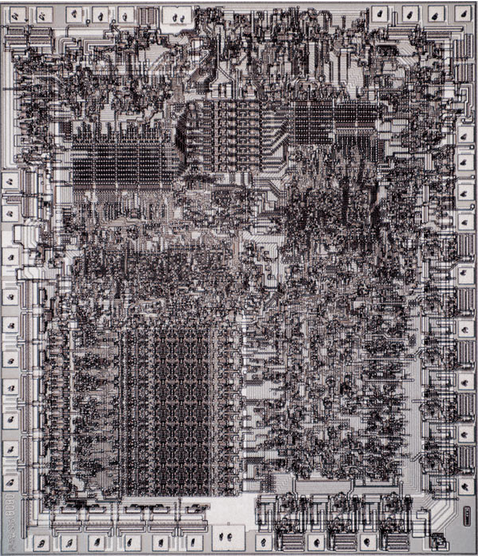
\includegraphics[height=4cm,width=4cm]{../present_figs/intel1974}
\caption{The Intel 8080 introduced in 1974 consisted of approximately 5,000 transistors}
\end{minipage}\hfill
\begin{minipage}{0.45\textwidth}
\centering
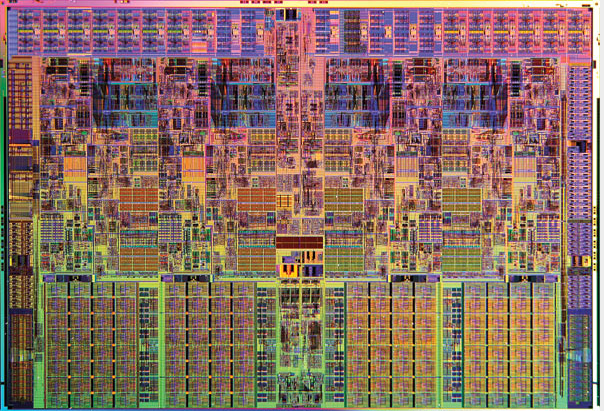
\includegraphics[height=4cm,width=4cm]{../present_figs/i7chip}
\caption{The Intel Core i7 in 2008 consisted of approximately 731 million transistors}
\end{minipage}
\end{figure}
\cite{Grifantini2008}
\end{frame}

\begin{frame}
\frametitle{Discovery of Graphene}
\end{frame}

\begin{frame}
\begin{figure}
\frametitle{Properties of Graphene}
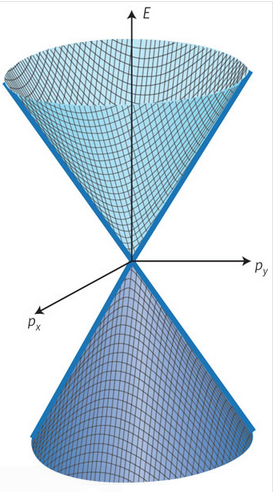
\includegraphics[height=6cm, width=3.75cm]{../present_figs/graphenebandgap}
\caption{Electronic band structure of graphene \cite{Fuhrer2010}.}
\end{figure}
\end{frame}

\section{\ch{MoS2} as Materials Beyond Graphene}
\begin{frame}
\frametitle{Transition Metal Dichalcogenides}

\begin{figure}
\centering
\begin{minipage}{0.45\textwidth}
\centering
\exedout % first figure itself
\caption{first figure}
\end{minipage}\hfill
\begin{minipage}{0.45\textwidth}
\centering
\exedout % second figure itself
\caption{second figure}
\end{minipage}
\end{figure}

\end{frame}

\begin{frame}
\frametitle{Properties of \ch{MoS2}}
\end{frame}

\begin{frame}
\frametitle{Micromechanical Exfoliation}
\end{frame}

\section{Applications of \ch{MoS2} in FETs}
\begin{frame}
\frametitle{\ch{MoS2} in FETs}
\end{frame}

\begin{frame}
\frametitle{\ch{MoS2} in FETs Continued}
\end{frame}

\section{Conclusion}
\begin{frame}
\frametitle{Outlook and Conclusion}
\end{frame}

\begin{frame}
\frametitle{References}
\footnotesize{
	\begin{thebibliography}{99}
	\bibitem[Fuhrer, 2010]{Fuhrer2010} Fuhrer, M.S. (2010)
	\newblock  Graphene: Ribbions piece-by-piece
	\newblock \emph{Nature Materials} (9), 611--612.

	\bibitem[Grifantini, 2008]{Grifantini2008} Grifantini, K. (2008)
	\newblock Moore's Law
	\newblock \emph{MIT Technology Review} \emph{http://www.technologyreview.com/photoessay/411485/moores-law/}.

	\end{thebibliography}
}
\end{frame}

%-----------------------------------------------------------------

\end{document} 